% vim: set spell spelllang=en tw=100 et sw=4 sts=4 foldmethod=marker foldmarker={{{,}}} :

\documentclass{beamer}

\usepackage{tikz}
\usepackage{xcolor}
\usepackage{complexity}
\usepackage{hyperref}
\usepackage{microtype}
\usepackage{amsmath}                   % \operatorname
\usepackage{amsfonts}                  % \mathcal
\usepackage{amssymb}                   % \nexists
\usepackage[vlined]{algorithm2e} % algorithms
\usepackage{centernot}
\usepackage{listings}
\usepackage{csquotes}

\RequirePackage[tt=false, type1=true]{libertine}
\RequirePackage[varqu]{zi4}
\RequirePackage[libertine]{newtxmath}
\RequirePackage[T1]{fontenc}

\usetikzlibrary{shapes, arrows, shadows, calc, positioning, fit}
\usetikzlibrary{decorations.pathreplacing, decorations.pathmorphing, shapes.misc}
\usetikzlibrary{tikzmark}

\definecolor{uofguniversityblue}{rgb}{0, 0.219608, 0.396078}

\definecolor{uofgheather}{rgb}{0.356863, 0.32549, 0.490196}
\definecolor{uofgaquamarine}{rgb}{0.603922, 0.72549, 0.678431}
\definecolor{uofgslate}{rgb}{0.309804, 0.34902, 0.380392}
\definecolor{uofgrose}{rgb}{0.823529, 0.470588, 0.709804}
\definecolor{uofgmocha}{rgb}{0.709804, 0.564706, 0.47451}
\definecolor{uofgsandstone}{rgb}{0.321569, 0.278431, 0.231373}
\definecolor{uofgforest}{rgb}{0, 0.2, 0.129412}
\definecolor{uofglawn}{rgb}{0.517647, 0.741176, 0}
\definecolor{uofgcobalt}{rgb}{0, 0.615686, 0.92549}
\definecolor{uofgturquoise}{rgb}{0, 0.709804, 0.819608}
\definecolor{uofgsunshine}{rgb}{1.0, 0.862745, 0.211765}
\definecolor{uofgpumpkin}{rgb}{1.0, 0.72549, 0.282353}
\definecolor{uofgthistle}{rgb}{0.584314, 0.070588, 0.447059}
\definecolor{uofgrust}{rgb}{0.603922, 0.227451, 0.023529}
\definecolor{uofgburgundy}{rgb}{0.490196, 0.133333, 0.223529}
\definecolor{uofgpillarbox}{rgb}{0.701961, 0.047059, 0}
\definecolor{uofglavendar}{rgb}{0.356863, 0.301961, 0.580392}

\tikzset{vertex/.style={draw, circle, inner sep=0pt, minimum size=0.5cm, font=\small\bfseries}}
\tikzset{notvertex/.style={vertex, color=white, text=black}}
\tikzset{plainvertex/.style={vertex}}
\tikzset{vertexc1/.style={vertex, fill=uofgburgundy, text=white}}
\tikzset{vertexc2/.style={vertex, fill=uofgsandstone, text=white}}
\tikzset{vertexc3/.style={vertex, fill=uofgforest, text=white}}
\tikzset{vertexc4/.style={vertex, fill=uofgheather, text=white}}
\tikzset{edge/.style={color=black!50!white}}
\tikzset{bedge/.style={ultra thick}}

% {{{ theme things
\useoutertheme[footline=authortitle]{miniframes}
\useinnertheme{rectangles}

\setbeamerfont{block title}{size={}}
\setbeamerfont{title}{size=\large,series=\bfseries}
\setbeamerfont{section title}{size=\large,series=\mdseries}
\setbeamerfont{author}{size=\normalsize,series=\mdseries}
\setbeamercolor*{structure}{fg=uofguniversityblue}
\setbeamercolor*{palette primary}{use=structure,fg=black,bg=white}
\setbeamercolor*{palette secondary}{use=structure,fg=white,bg=uofgcobalt}
\setbeamercolor*{palette tertiary}{use=structure,fg=white,bg=uofguniversityblue}
\setbeamercolor*{palette quaternary}{fg=white,bg=black}

\setbeamercolor*{titlelike}{parent=palette primary}

\beamertemplatenavigationsymbolsempty

\setbeamertemplate{title page}
{
    \begin{tikzpicture}[remember picture, overlay]
        \node at (current page.north west) {
            \begin{tikzpicture}[remember picture, overlay]
                \fill [fill=uofguniversityblue, anchor=north west] (0, 0) rectangle (\paperwidth, -2.2cm);
            \end{tikzpicture}
        };

        \node (logo) [anchor=north east, shift={(-0.6cm,-0.4cm)}] at (current page.north east) {
            
\includegraphics[keepaspectratio=true,scale=0.7]{UoG_keyline.pdf}
        };

        \node [anchor=west, xshift=0.2cm] at (current page.west |- logo.west) {
            \begin{minipage}{0.7\paperwidth}\raggedright
                {\usebeamerfont{title}\usebeamercolor[white]{}\inserttitle}\\[0.1cm]
                {\usebeamerfont{author}\usebeamercolor[white]{}\insertauthor}
            \end{minipage}
        };
    \end{tikzpicture}
}

\setbeamertemplate{section page}
{
    \begin{centering}
        \begin{beamercolorbox}[sep=12pt,center]{part title}
            \usebeamerfont{section title}\insertsection\par
        \end{beamercolorbox}
    \end{centering}
}

\newcommand{\frameofframes}{/}
\newcommand{\setframeofframes}[1]{\renewcommand{\frameofframes}{#1}}

\makeatletter
\setbeamertemplate{footline}
{%
    \begin{beamercolorbox}[colsep=1.5pt]{upper separation line foot}
    \end{beamercolorbox}
    \begin{beamercolorbox}[ht=2.5ex,dp=1.125ex,%
        leftskip=.3cm,rightskip=.3cm plus1fil]{author in head/foot}%
        \leavevmode{\usebeamerfont{author in head/foot}\insertshortauthor}%
        \hfill%
        {\usebeamerfont{institute in head/foot}\usebeamercolor[fg]{institute in head/foot}\insertshortinstitute}%
    \end{beamercolorbox}%
    \begin{beamercolorbox}[ht=2.5ex,dp=1.125ex,%
        leftskip=.3cm,rightskip=.3cm plus1fil]{title in head/foot}%
        {\usebeamerfont{title in head/foot}\insertshorttitle}%
        \hfill%
        {\usebeamerfont{frame number}\usebeamercolor[fg]{frame number}\insertframenumber~\frameofframes~\inserttotalframenumber}
    \end{beamercolorbox}%
    \begin{beamercolorbox}[colsep=1.5pt]{lower separation line foot}
    \end{beamercolorbox}
}

\makeatletter
\newenvironment{nearlyplainframe}[2][]{
    \def\beamer@entrycode{\vspace*{-\headheight}\vspace*{3pt}}
    \setbeamertemplate{headline}
    {%
        \begin{beamercolorbox}[colsep=1.5pt]{upper separation line head}
        \end{beamercolorbox}
        \begin{beamercolorbox}[ht=0.5ex,dp=0.125ex,%
            leftskip=.3cm,rightskip=.3cm plus1fil]{title in head/foot}%
        \end{beamercolorbox}%
        \begin{beamercolorbox}[ht=0.5ex,dp=0.125ex,%
            leftskip=.3cm,rightskip=.3cm plus1fil]{author in head/foot}%
        \end{beamercolorbox}%
        \begin{beamercolorbox}[colsep=1.5pt]{lower separation line head}
        \end{beamercolorbox}
        \vspace*{\headheight}
    }

    \setbeamertemplate{footline}
    {%
        \begin{beamercolorbox}[colsep=1.5pt]{upper separation line foot}
        \end{beamercolorbox}
        \begin{beamercolorbox}[ht=0.5ex,dp=0.125ex,%
            leftskip=.3cm,rightskip=.3cm plus1fil]{author in head/foot}%
        \end{beamercolorbox}%
        \begin{beamercolorbox}[ht=0.5ex,dp=0.125ex,%
            leftskip=.3cm,rightskip=.3cm plus1fil]{title in head/foot}%
        \end{beamercolorbox}%
        \begin{beamercolorbox}[colsep=1.5pt]{lower separation line foot}
        \end{beamercolorbox}
    }

    \begin{frame}[#1]{#2}
    }{
    \end{frame}
}
\makeatother

\makeatletter
\newenvironment{justborderframe}[2][]{
    \def\beamer@entrycode{\vspace*{-\headheight}}
    \setbeamertemplate{headline}
    {%
        \begin{beamercolorbox}[colsep=1.5pt]{upper separation line head}
        \end{beamercolorbox}
        \begin{beamercolorbox}[ht=0.5ex,dp=0.125ex,%
            leftskip=.3cm,rightskip=.3cm plus1fil]{title in head/foot}%
        \end{beamercolorbox}%
        \begin{beamercolorbox}[ht=0.5ex,dp=0.125ex,%
            leftskip=.3cm,rightskip=.3cm plus1fil]{author in head/foot}%
        \end{beamercolorbox}%
        \begin{beamercolorbox}[colsep=1.5pt]{lower separation line head}
        \end{beamercolorbox}
        \vspace*{\headheight}
    }

    \setbeamertemplate{footline}
    {%
        \begin{beamercolorbox}[colsep=1.5pt]{upper separation line foot}
        \end{beamercolorbox}
        \begin{beamercolorbox}[ht=0.5ex,dp=0.125ex,%
            leftskip=.3cm,rightskip=.3cm plus1fil]{author in head/foot}%
        \end{beamercolorbox}%
        \begin{beamercolorbox}[ht=0.5ex,dp=0.125ex,%
            leftskip=.3cm,rightskip=.3cm plus1fil]{title in head/foot}%
        \end{beamercolorbox}%
        \begin{beamercolorbox}[colsep=1.5pt]{lower separation line foot}
        \end{beamercolorbox}
    }

    \begin{frame}[#1]{}
    }{
    \end{frame}
}
\makeatother


% }}}

\author[Ciaran McCreesh]{Ciaran McCreesh}
\title{Are ``Hard'' Subgraph Problems Hard?}

\begin{document}

{
    \usebackgroundtemplate{
        \tikz[overlay, remember picture]
        \node[at=(current page.south), anchor=south, inner sep=0pt]{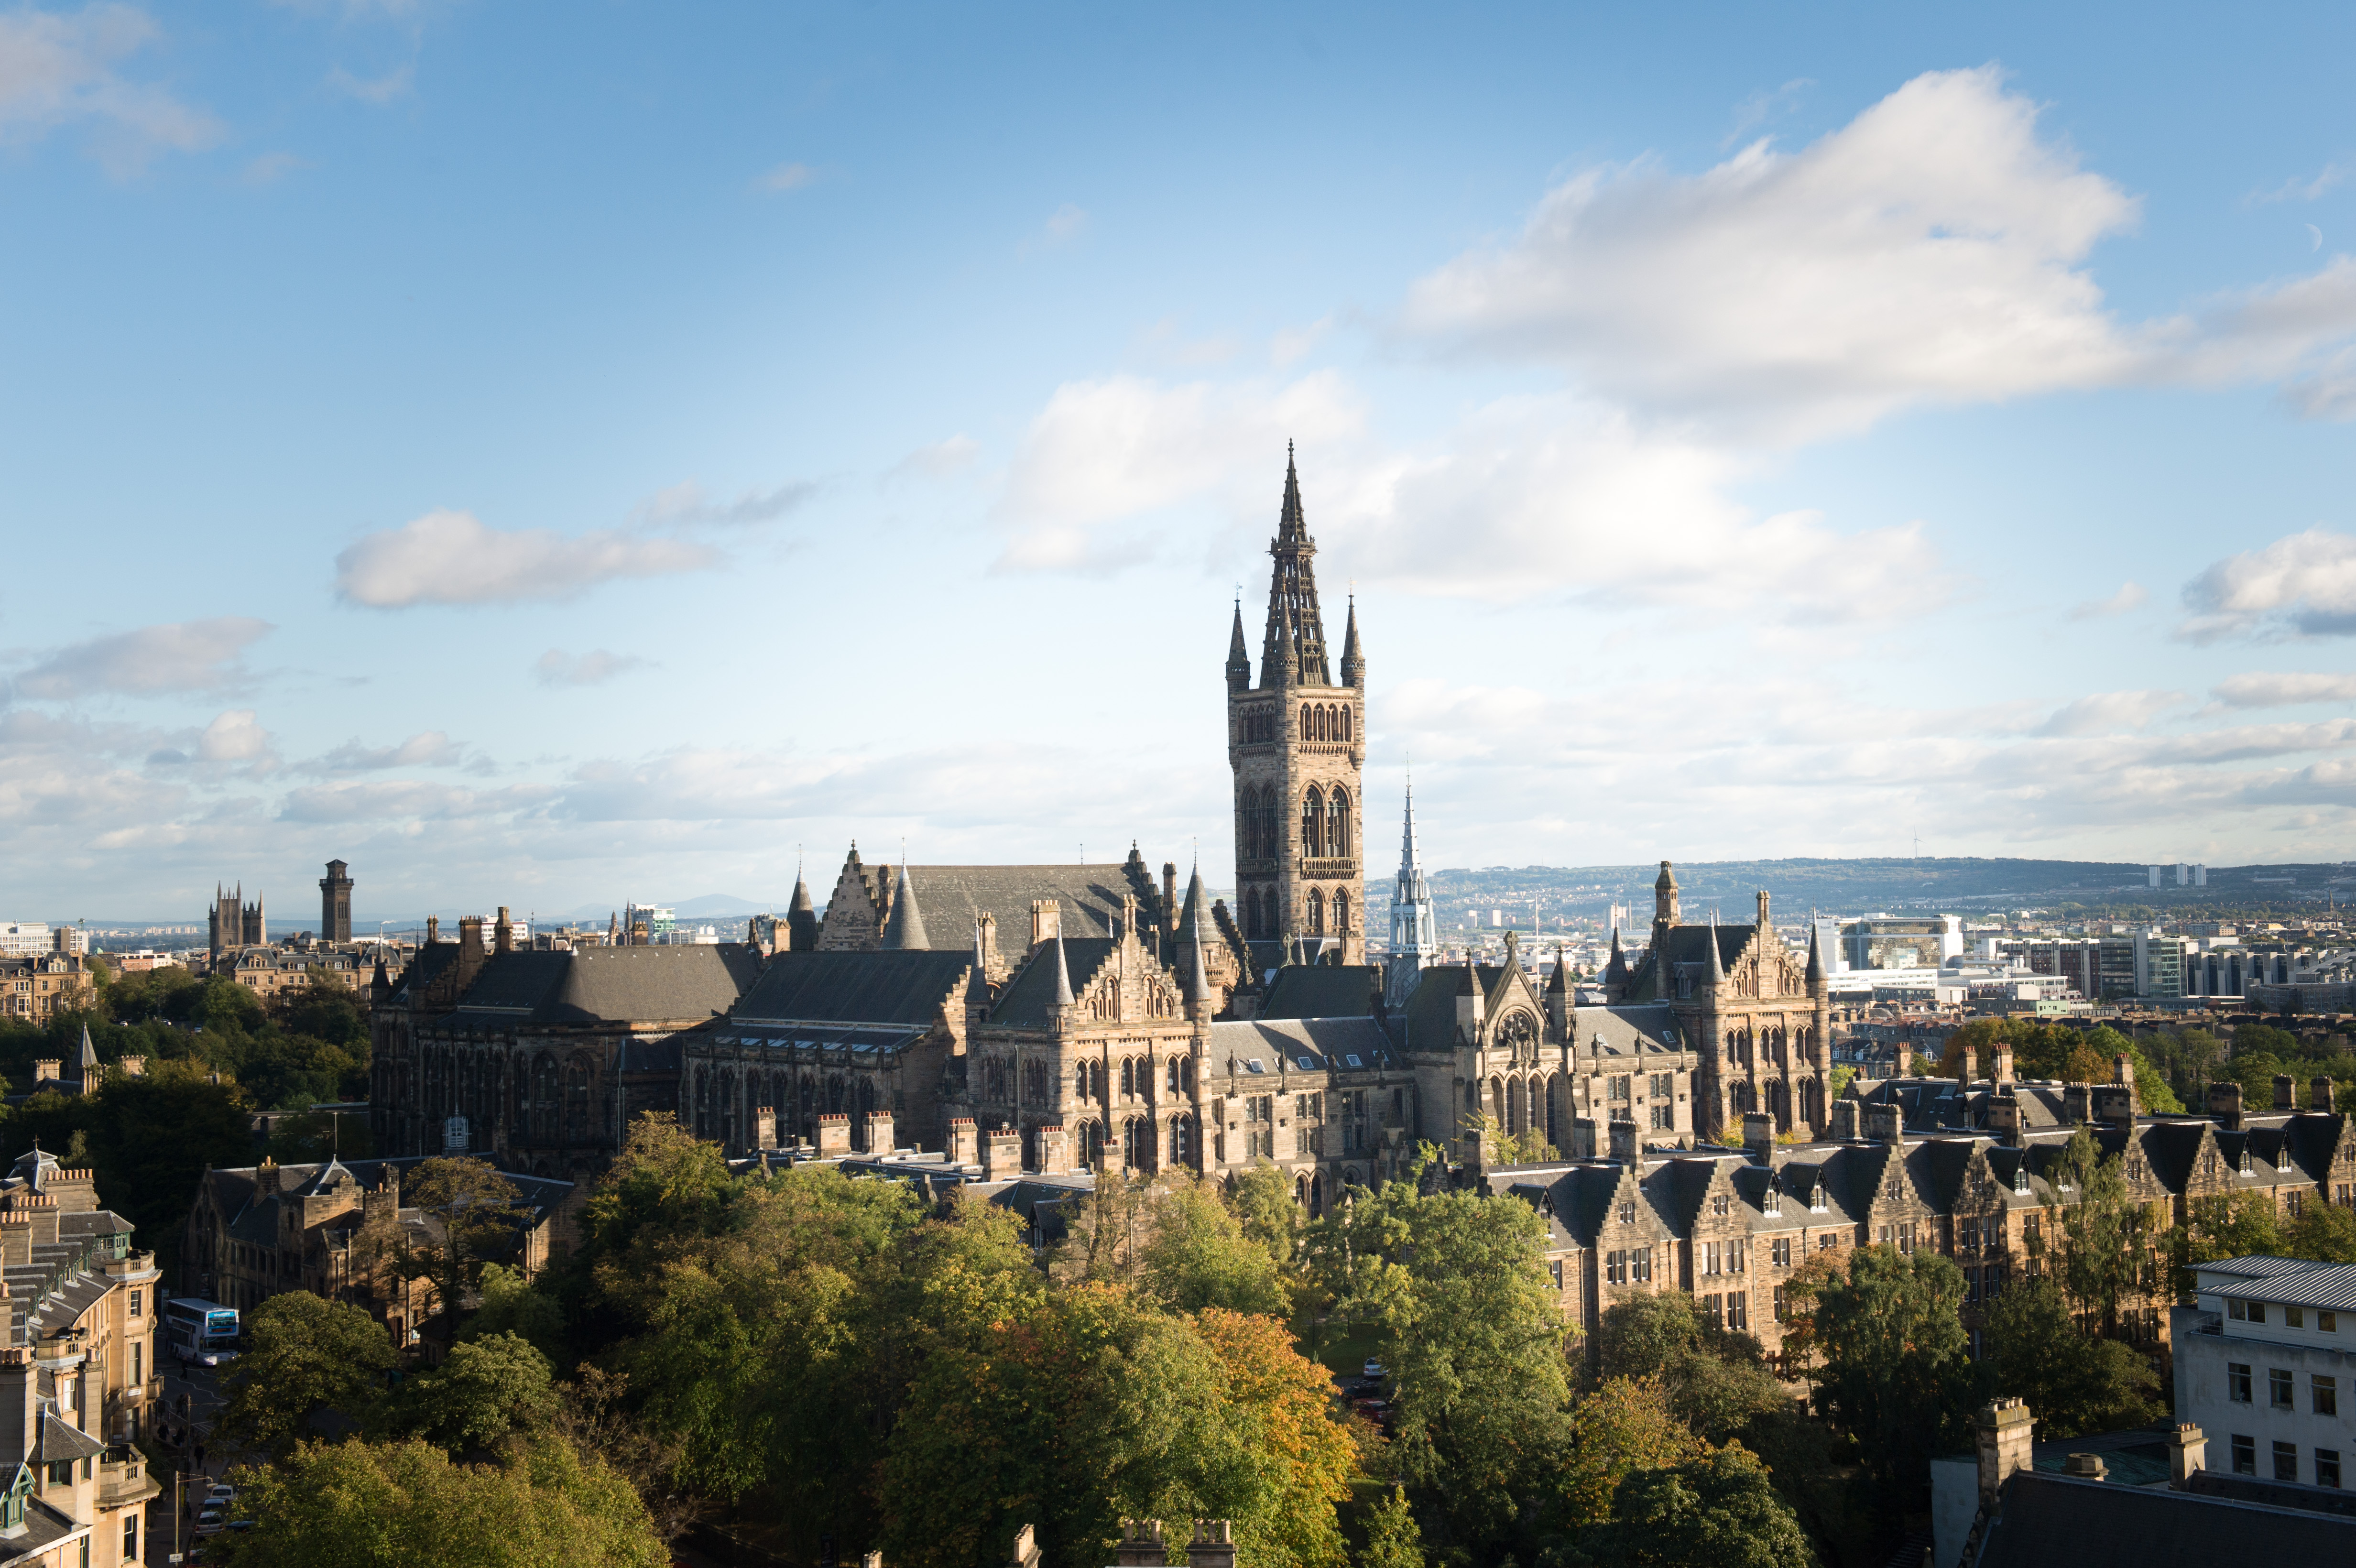
\includegraphics[keepaspectratio=true, height=\paperheight]{background.jpg}};
    }
    \begin{frame}[plain,noframenumbering]
        \titlepage
    \end{frame}
}

\section{Graph Problems}

\begin{frame}{Subgraph Isomorphism}
    \centering
    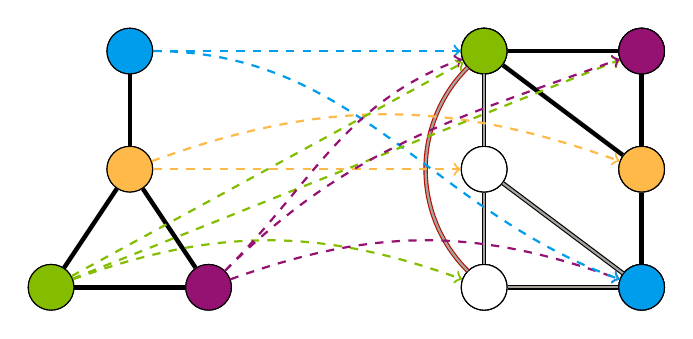
\begin{tikzpicture}
        \node <1> [draw, circle, fill=white, inner sep=4pt, font=\bfseries] (Na) at (1,  0) {\vphantom{1}};
        \node <1> [draw, circle, fill=white, inner sep=4pt, font=\bfseries] (Nb) at (1, -1.5) {\vphantom{1}};
        \node <1> [draw, circle, fill=white, inner sep=4pt, font=\bfseries] (Nc) at (0, -3) {\vphantom{1}};
        \node <1> [draw, circle, fill=white, inner sep=4pt, font=\bfseries] (Nd) at (2, -3) {\vphantom{1}};

        \node <2-5> [draw, circle, fill=uofgcobalt, inner sep=4pt, font=\bfseries] (Na) at (1,  0) {\vphantom{1}};
        \node <2-5> [draw, circle, fill=uofgpumpkin, inner sep=4pt, font=\bfseries] (Nb) at (1, -1.5) {\vphantom{1}};
        \node <2-5> [draw, circle, fill=uofglawn, inner sep=4pt, font=\bfseries] (Nc) at (0, -3) {\vphantom{1}};
        \node <2-5> [draw, circle, fill=uofgthistle, inner sep=4pt, font=\bfseries] (Nd) at (2, -3) {\vphantom{1}};

        \draw [ultra thick] (Na) -- (Nb);
        \draw [ultra thick] (Nb) -- (Nc);
        \draw [ultra thick] (Nc) -- (Nd);
        \draw [ultra thick] (Nb) -- (Nd);

        \node <1> [draw, circle, fill=white, inner sep=4pt, font=\bfseries] (N1) at (5.5,  0) {\vphantom{1}};
        \node <1> [draw, circle, fill=white, inner sep=4pt, font=\bfseries] (N2) at (7.5,  0) {\vphantom{1}};
        \node <1> [draw, circle, fill=white, inner sep=4pt, font=\bfseries] (N3) at (5.5, -1.5) {\vphantom{1}};
        \node <1> [draw, circle, fill=white, inner sep=4pt, font=\bfseries] (N4) at (7.5, -1.5) {\vphantom{1}};
        \node <1> [draw, circle, fill=white, inner sep=4pt, font=\bfseries] (N5) at (5.5, -3) {\vphantom{1}};
        \node <1> [draw, circle, fill=white, inner sep=4pt, font=\bfseries] (N6) at (7.5, -3) {\vphantom{1}};

        \node <2-3> [draw, circle, fill=uofgcobalt, inner sep=4pt, font=\bfseries] (N1) at (5.5,  0) {\vphantom{1}};
        \node <2-3> [draw, circle, fill=white, inner sep=4pt, font=\bfseries] (N2) at (7.5,  0) {\vphantom{1}};
        \node <2-3> [draw, circle, fill=uofgpumpkin, inner sep=4pt, font=\bfseries] (N3) at (5.5, -1.5) {\vphantom{1}};
        \node <2-3> [draw, circle, fill=white, inner sep=4pt, font=\bfseries] (N4) at (7.5, -1.5) {\vphantom{1}};
        \node <2-3> [draw, circle, fill=uofglawn, inner sep=4pt, font=\bfseries] (N5) at (5.5, -3) {\vphantom{1}};
        \node <2-3> [draw, circle, fill=uofgthistle, inner sep=4pt, font=\bfseries] (N6) at (7.5, -3) {\vphantom{1}};

        \node <5> [draw, circle, fill=uofgthistle, inner sep=4pt, font=\bfseries] (N1) at (5.5,  0) {\vphantom{1}};
        \node <5> [draw, circle, fill=uofglawn, inner sep=4pt, font=\bfseries] (N2) at (7.5,  0) {\vphantom{1}};
        \node <4> [draw, circle, fill=uofglawn, inner sep=4pt, font=\bfseries] (N1) at (5.5,  0) {\vphantom{1}};
        \node <4> [draw, circle, fill=uofgthistle, inner sep=4pt, font=\bfseries] (N2) at (7.5,  0) {\vphantom{1}};
        \node <4-5> [draw, circle, fill=white, inner sep=4pt, font=\bfseries] (N3) at (5.5, -1.5) {\vphantom{1}};
        \node <4-5> [draw, circle, fill=uofgpumpkin, inner sep=4pt, font=\bfseries] (N4) at (7.5, -1.5) {\vphantom{1}};
        \node <4-5> [draw, circle, fill=white, inner sep=4pt, font=\bfseries] (N5) at (5.5, -3) {\vphantom{1}};
        \node <4-5> [draw, circle, fill=uofgcobalt, inner sep=4pt, font=\bfseries] (N6) at (7.5, -3) {\vphantom{1}};

        \draw <1> [thick, color=uofgsandstone!50] (N1) -- (N2);
        \draw <1> [thick, color=uofgsandstone!50] (N1) -- (N3);
        \draw <1> [thick, color=uofgsandstone!50] (N1) -- (N4);
        \draw <1> [thick, color=uofgsandstone!50] (N2) -- (N4);
        \draw <1> [thick, color=uofgsandstone!50] (N3) -- (N5);
        \draw <1> [thick, color=uofgsandstone!50] (N3) -- (N6);
        \draw <1> [thick, color=uofgsandstone!50] (N4) -- (N6);
        \draw <1> [thick, color=uofgsandstone!50] (N5) -- (N6);
        \draw <1> [thick, color=uofgsandstone!50] (N1) to [in=135, out=225] (N5);

        \draw <2-3> [thick, color=uofgsandstone!50] (N1) -- (N2);
        \draw <2-3> [ultra thick] (N1) -- (N3);
        \draw <2-3> [thick, color=uofgsandstone!50] (N1) -- (N4);
        \draw <2-3> [thick, color=uofgsandstone!50] (N2) -- (N4);
        \draw <2-3> [ultra thick] (N3) -- (N5);
        \draw <2-3> [ultra thick] (N3) -- (N6);
        \draw <2-3> [thick, color=uofgsandstone!50] (N4) -- (N6);
        \draw <2-3> [ultra thick] (N5) -- (N6);
        \draw <2> [thick, color=uofgsandstone!50] (N1) to [in=135, out=225] (N5);
        \draw <3> [ultra thick, color=uofgpillarbox] (N1) to [in=135, out=225] (N5);

        \draw <4-5> [ultra thick] (N1) -- (N2);
        \draw <4-5> [thick, color=uofgsandstone!50] (N1) -- (N3);
        \draw <4-5> [ultra thick] (N1) -- (N4);
        \draw <4-5> [ultra thick] (N2) -- (N4);
        \draw <4-5> [thick, color=uofgsandstone!50] (N3) -- (N5);
        \draw <4-5> [thick, color=uofgsandstone!50] (N3) -- (N6);
        \draw <4-5> [ultra thick] (N4) -- (N6);
        \draw <4-5> [thick, color=uofgsandstone!50] (N5) -- (N6);
        \draw <4-5> [thick, color=uofgsandstone!50] (N1) to [in=135, out=225] (N5);

        \draw <2-3> [thick, dashed, color=uofgcobalt, arrows=->] (Na) to (N1);
        \draw <2-3> [thick, dashed, color=uofgpumpkin, arrows=->] (Nb) to (N3);
        \draw <2-3> [thick, dashed, color=uofglawn, arrows=->] (Nc) to [out=20, in=160] (N5);
        \draw <2-3> [thick, dashed, color=uofgthistle, arrows=->] (Nd) to [out=20, in=160] (N6);

        \draw <4-5> [thick, dashed, color=uofgcobalt, arrows=->] (Na) to [out=0, in=160] (N6);
        \draw <4-5> [thick, dashed, color=uofgpumpkin, arrows=->] (Nb) to [out=20, in=160] (N4);
        \draw <5> [thick, dashed, color=uofglawn, arrows=->] (Nc) to (N2);
        \draw <5> [thick, dashed, color=uofgthistle, arrows=->] (Nd) to [in=200] (N1);
        \draw <4> [thick, dashed, color=uofglawn, arrows=->] (Nc) to (N1);
        \draw <4> [thick, dashed, color=uofgthistle, arrows=->] (Nd) to [in=200] (N2);
    \end{tikzpicture}
\end{frame}

\begin{frame}{Maximum Common Induced Subgraph}
    \centering
    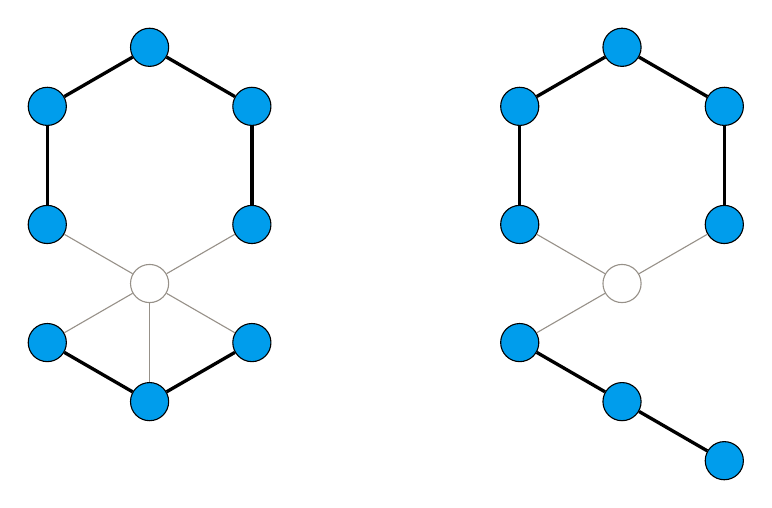
\begin{tikzpicture}
        \begin{scope}
            \node[draw, circle, fill=uofgcobalt, inner sep=2pt, font=\normalsize] (M1) at (90:1.5) {\phantom{0}};
            \node[draw, circle, fill=uofgcobalt, inner sep=2pt, font=\normalsize] (M2) at (150:1.5) {\phantom{0}};
            \node[draw, circle, fill=uofgcobalt, inner sep=2pt, font=\normalsize] (M3) at (30:1.5) {\phantom{0}};
            \node[draw, circle, fill=uofgcobalt, inner sep=2pt, font=\normalsize] (M4) at (210:1.5) {\phantom{0}};
            \node[draw, circle, fill=uofgcobalt, inner sep=2pt, font=\normalsize] (M5) at (330:1.5) {\phantom{0}};
            \node[draw, circle, draw=uofgsandstone!60, fill=white, inner sep=2pt, font=\normalsize] (M6) at (270:1.5) {\phantom{0}};
            \node[draw, circle, fill=uofgcobalt, inner sep=2pt, font=\normalsize] (M7) at ($(210:1.5) + (M6)$) {\phantom{0}};
            \node[draw, circle, fill=uofgcobalt, inner sep=2pt, font=\normalsize] (M8) at ($(330:1.5) + (M6)$) {\phantom{0}};
            \node[draw, circle, fill=uofgcobalt, inner sep=2pt, font=\normalsize] (M9) at ($(270:1.5) + (M6)$) {\phantom{0}};

            \draw [very thick] (M1) -- (M2);
            \draw [very thick] (M2) -- (M4);
            \draw [very thick] (M3) -- (M5);
            \draw [color=uofgsandstone!60] (M4) -- (M6);
            \draw [color=uofgsandstone!60] (M5) -- (M6);
            \draw [very thick] (M3) -- (M1);
            \draw [color=uofgsandstone!60] (M6) -- (M7);
            \draw [color=uofgsandstone!60] (M6) -- (M8);
            \draw [color=uofgsandstone!60] (M6) -- (M9);
            \draw [very thick] (M7) -- (M9);
            \draw [very thick] (M8) -- (M9);
        \end{scope}

        \begin{scope}[xshift=6cm]
            \node[draw, circle, fill=uofgcobalt, inner sep=2pt, font=\normalsize] (M1) at (90:1.5) {\phantom{0}};
            \node[draw, circle, fill=uofgcobalt, inner sep=2pt, font=\normalsize] (M2) at (150:1.5) {\phantom{0}};
            \node[draw, circle, fill=uofgcobalt, inner sep=2pt, font=\normalsize] (M3) at (30:1.5) {\phantom{0}};
            \node[draw, circle, fill=uofgcobalt, inner sep=2pt, font=\normalsize] (M4) at (210:1.5) {\phantom{0}};
            \node[draw, circle, fill=uofgcobalt, inner sep=2pt, font=\normalsize] (M5) at (330:1.5) {\phantom{0}};
            \node[draw, circle, draw=uofgsandstone!60, fill=white, inner sep=2pt, font=\normalsize] (M6) at (270:1.5) {\phantom{0}};
            \node[draw, circle, fill=uofgcobalt, inner sep=2pt, font=\normalsize] (M7) at ($(210:1.5) + (M6)$) {\phantom{0}};
            \node[draw, circle, fill=uofgcobalt, inner sep=2pt, font=\normalsize] (M8) at ($(270:1.5) + (M6)$) {\phantom{0}};
            \node[draw, circle, fill=uofgcobalt, inner sep=2pt, font=\normalsize] (M9) at ($(330:1.5) + (M8)$) {\phantom{0}};

            \draw [very thick] (M1) -- (M2);
            \draw [very thick] (M2) -- (M4);
            \draw [very thick] (M3) -- (M5);
            \draw [color=uofgsandstone!60] (M4) -- (M6);
            \draw [color=uofgsandstone!60] (M5) -- (M6);
            \draw [very thick] (M3) -- (M1);
            \draw [color=uofgsandstone!60] (M6) -- (M7);
            \draw [very thick] (M7) -- (M8);
            \draw [very thick] (M8) -- (M9);
        \end{scope}
    \end{tikzpicture}
\end{frame}

\begin{frame}{Maximum Common Induced Connected Subgraph}
    \centering
    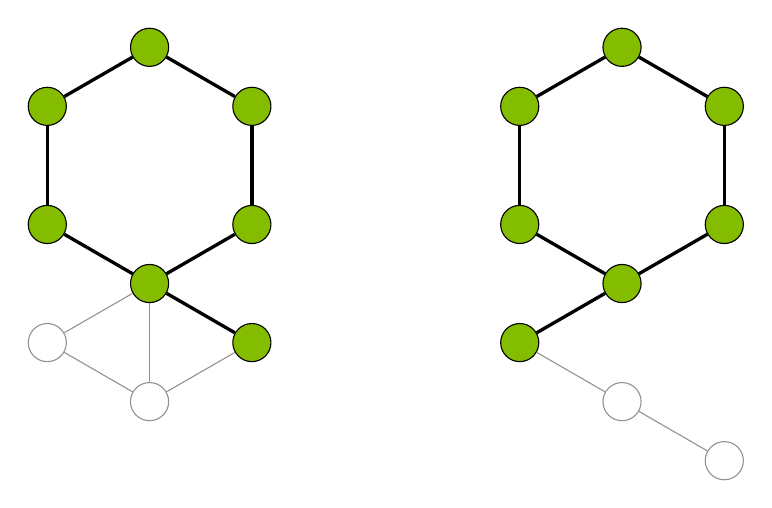
\begin{tikzpicture}
        \begin{scope}
            \node[draw, circle, fill=uofglawn, inner sep=2pt, font=\normalsize] (M1) at (90:1.5) {\phantom{0}};
            \node[draw, circle, fill=uofglawn, inner sep=2pt, font=\normalsize] (M2) at (150:1.5) {\phantom{0}};
            \node[draw, circle, fill=uofglawn, inner sep=2pt, font=\normalsize] (M3) at (30:1.5) {\phantom{0}};
            \node[draw, circle, fill=uofglawn, inner sep=2pt, font=\normalsize] (M4) at (210:1.5) {\phantom{0}};
            \node[draw, circle, fill=uofglawn, inner sep=2pt, font=\normalsize] (M5) at (330:1.5) {\phantom{0}};
            \node[draw, circle, fill=uofglawn, inner sep=2pt, font=\normalsize] (M6) at (270:1.5) {\phantom{0}};
            \node[draw, circle, draw=uofgsandstone!60, fill=white, inner sep=2pt, font=\normalsize] (M7) at ($(210:1.5) + (M6)$) {\phantom{0}};
            \node[draw, circle, fill=uofglawn, inner sep=2pt, font=\normalsize] (M8) at ($(330:1.5) + (M6)$) {\phantom{0}};
            \node[draw, circle, draw=uofgsandstone!60, fill=white, inner sep=2pt, font=\normalsize] (M9) at ($(270:1.5) + (M6)$) {\phantom{0}};

            \draw [very thick] (M1) -- (M2);
            \draw [very thick] (M2) -- (M4);
            \draw [very thick] (M3) -- (M5);
            \draw [very thick] (M4) -- (M6);
            \draw [very thick] (M5) -- (M6);
            \draw [very thick] (M3) -- (M1);
            \draw [color=uofgsandstone!60] (M6) -- (M7);
            \draw [very thick] (M6) -- (M8);
            \draw [color=uofgsandstone!60] (M6) -- (M9);
            \draw [color=uofgsandstone!60] (M7) -- (M9);
            \draw [color=uofgsandstone!60] (M8) -- (M9);
        \end{scope}

        \begin{scope}[xshift=6cm]
            \node[draw, circle, fill=uofglawn, inner sep=2pt, font=\normalsize] (M1) at (90:1.5) {\phantom{0}};
            \node[draw, circle, fill=uofglawn, inner sep=2pt, font=\normalsize] (M2) at (150:1.5) {\phantom{0}};
            \node[draw, circle, fill=uofglawn, inner sep=2pt, font=\normalsize] (M3) at (30:1.5) {\phantom{0}};
            \node[draw, circle, fill=uofglawn, inner sep=2pt, font=\normalsize] (M4) at (210:1.5) {\phantom{0}};
            \node[draw, circle, fill=uofglawn, inner sep=2pt, font=\normalsize] (M5) at (330:1.5) {\phantom{0}};
            \node[draw, circle, fill=uofglawn, inner sep=2pt, font=\normalsize] (M6) at (270:1.5) {\phantom{0}};
            \node[draw, circle, fill=uofglawn, inner sep=2pt, font=\normalsize] (M7) at ($(210:1.5) + (M6)$) {\phantom{0}};
            \node[draw, circle, draw=uofgsandstone!60, fill=white, inner sep=2pt, font=\normalsize] (M8) at ($(270:1.5) + (M6)$) {\phantom{0}};
            \node[draw, circle, draw=uofgsandstone!60, fill=white, inner sep=2pt, font=\normalsize] (M9) at ($(330:1.5) + (M8)$) {\phantom{0}};

            \draw [very thick] (M1) -- (M2);
            \draw [very thick] (M2) -- (M4);
            \draw [very thick] (M3) -- (M5);
            \draw [very thick] (M4) -- (M6);
            \draw [very thick] (M5) -- (M6);
            \draw [very thick] (M3) -- (M1);
            \draw [very thick] (M6) -- (M7);
            \draw [draw=uofgsandstone!60] (M7) -- (M8);
            \draw [draw=uofgsandstone!60] (M8) -- (M9);
        \end{scope}
    \end{tikzpicture}
\end{frame}

\begin{frame}{Maximum Clique}
    \centering
    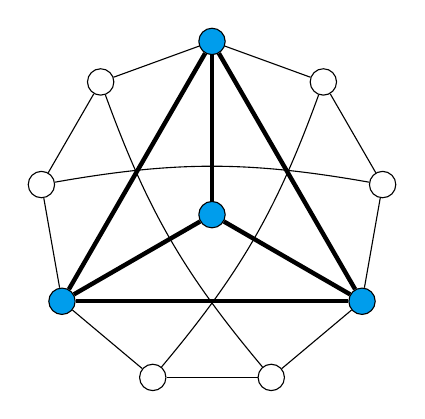
\begin{tikzpicture}
        \newcount \myc
        \foreach \n in {1, ..., 9}{
            \myc=\n \advance\myc by -1 \multiply\myc by -360 \divide\myc by 9 \advance\myc by 290.0
            \ifthenelse{\n = 3 \OR \n = 6 \OR \n = 9}{
                \node[draw, circle, fill=uofgcobalt, inner sep=0.5pt] (N\n) at (\the\myc:2.2) {\phantom{0}};
            }{
                \node[draw, circle, fill=white, inner sep=0.5pt] (N\n) at (\the\myc:2.2) {\phantom{0}};
            }
        }
        \node[draw, circle, fill=uofgcobalt, inner sep=0.5pt] (N10) at (0, 0) {\phantom{0}};

        \draw (N1) -- (N2);
        \draw (N2) -- (N3);
        \draw (N3) -- (N4);
        \draw (N4) -- (N5);
        \draw (N5) -- (N6);
        \draw (N6) -- (N7);
        \draw (N7) -- (N8);
        \draw (N8) -- (N9);
        \draw (N9) -- (N1);

        \draw (N4) to [out=10, in=170] (N8);
        \draw (N2) to [out=50, in=250] (N7);
        \draw (N5) to [out=290, in=130] (N1);

        \draw [ultra thick] (N3) -- (N10);
        \draw [ultra thick] (N6) -- (N10);
        \draw [ultra thick] (N9) -- (N10);
        \draw [ultra thick] (N6) -- (N3);
        \draw [ultra thick] (N9) -- (N3);
        \draw [ultra thick] (N6) -- (N9);
    \end{tikzpicture}
\end{frame}

\begin{frame}{Who Cares?}
    \begin{itemize}
        \item Chemistry, biochemistry, and drug design (graphs are molecule fragments or proteins).
        \item Computer vision.
        \item Compilers (instruction generation, code rewriting).
        \item Plagiarism and malware detection.
        \item Livestock epidemiology (contact and trade graphs).
        \item Designing mechanical lock systems.
    \end{itemize}
\end{frame}

\begin{frame}{In Theory\ldots}
    \begin{itemize}
        \item Subgraph finding is hard.
        \item Subgraph counting is hard.
        \item Approximate subgraph finding is hard.
    \end{itemize}
\end{frame}

\begin{frame}{In Practice\ldots}
    \begin{itemize}
        \item We have good \emph{solvers} for subgraph problems.
        \item Some applications involve solving thousands of subgraph isomorphism queries per second.
        \item We can solve clique on larger graphs than we can solve all-pairs
            shortest path.\footnote{Terms and conditions apply.}
    \end{itemize}
\end{frame}

\section{Graph Solvers}

\begin{frame}{Popular Families of Subgraph Isomorphism Algorithms}
    \begin{itemize}
        \item Connectivity-based:
            \begin{itemize}
                \item VF2 (2004), VF3 (2017)
                \item RI (2013)
            \end{itemize}
        \item Constraint programming:
            \begin{itemize}
                \item Ullman (1976)
                \item LAD (AIJ 2010), SND (CP 2014), PathLAD (LION 2016)
                \item Glasgow (CP 2015, LION 2016, CPAIOR 2019, \ldots)
            \end{itemize}
    \end{itemize}
\end{frame}

\begin{frame}{Benchmark Instances}

    \begin{itemize}
        \item 14,621 instances from Christine Solnon's collection:
            \begin{itemize}
                \item Randomly generated with different models.
                \item Real-world graphs.
                \item Computer vision problems.
                \item Biochemistry problems.
                \item Phase transition instances.
            \end{itemize}
        \item At least\ldots
            \begin{itemize}
                \item $\ge$ 2,110 satisfiable.
                \item $\ge$ 12,322 unsatisfiable.
            \end{itemize}
        \item A lot of them are very easy for good algorithms.
    \end{itemize}

\end{frame}

\begin{frame}{Horse Race!}

    \includegraphics<1>{gen-graph-others.pdf}%

\end{frame}

\begin{frame}{Easy Conclusion!}
    \begin{itemize}
        \item CP is best!
    \end{itemize}
\end{frame}

\begin{frame}{An Observation about Certain Datasets}
    \begin{itemize}
        \item All of the randomly generated instances from the MIVIA suites are satisfiable.
        \item The target graphs are randomly generated, and patterns are made by selecting
            random connected subgraphs and permuting them.
        \item These instances are usually rather easy\ldots
        \item Many papers use \emph{only} these instances for benchmarking.
    \end{itemize}
\end{frame}

\begin{frame}{A Different Easy Conclusion!}
    \begin{itemize}
        \item CP is slow! RI is best!
    \end{itemize}
\end{frame}

\section{The Glasgow Solver}

\begin{frame}{A Quick Introduction to Constraint Programming}
    \begin{itemize}
        \item A declarative way of describing (hard) problems.
        \item A set of variables, each of which has a (finite) domain of values.
        \item A set of constraints (in any form we like, so arbitrary arity, non-linear, etc).
        \item Combining inference and clever backtracking search, give each variable a value from its
            domain, such that all constraints are respected.
    \end{itemize}
\end{frame}

\begin{frame}{Subgraph Finding, as a Constraint Program}
    \begin{itemize}
        \item A variable for each pattern vertex. The domains are all of the target vertices.
        \item At least two sets of constraints:
            \begin{itemize}
                \item Adjacent pairs of vertices must be mapped to adjacent pairs of vertices.
                \item Injectivity, known as ``all different''.
            \end{itemize}
    \end{itemize}
\end{frame}

\begin{frame}{The Glasgow Subgraph Solver}
    \begin{center}
        \url{https://github.com/ciaranm/glasgow-subgraph-solver}
    \end{center}

    \begin{itemize}
        \item Subgraph isomorphism, and all its variants (induced / non-induced, homomorphism,
            locally injective, labels, side constraints, directed, \ldots).
        \item Also special algorithms for clique.
    \end{itemize}
\end{frame}

\begin{frame}{Some Clever Things We Can Deduce About Graphs}
    \begin{itemize}
        \item A pattern vertex of degree $k$ cannot be mapped to a target vertex of degree $k - 1$
            or smaller.
            \begin{itemize}
                \item We can also reason about neighbourhood degree sequences.
            \end{itemize}
        \item Two pattern vertices that are distance $d$ apart cannot be mapped to a pair of target
            vertices that are further than $d$ apart.
            \begin{itemize}
                \item We can also reason about the number of distinct short simple paths between two
                    vertices.
            \end{itemize}
        \item Search by branching on the smallest domain first, tie-breaking on the highest degree,
            and start by trying the highest degree target vertex first.
            \begin{itemize}
                \item Then do more sneaky things involving slight randomisation, restarts, parallel
                    search, \ldots
            \end{itemize}
        \item If we have a clique subproblem, do something else.
    \end{itemize}
\end{frame}

\section{Empirical Hardness}

\begin{frame}{Is Clique-Finding Hard?}
    \centering
    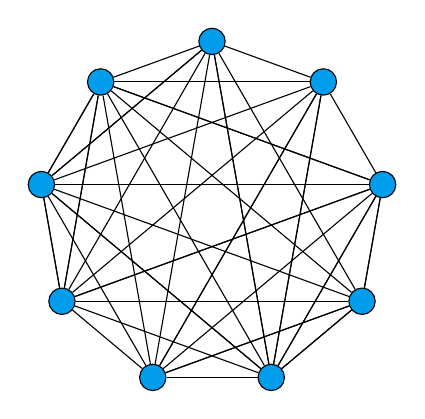
\begin{tikzpicture}
        \newcount \myc
        \foreach \n in {1, ..., 9}{
            \myc=\n \advance\myc by -1 \multiply\myc by -360 \divide\myc by 9 \advance\myc by 290.0
            \node[draw, circle, fill=uofgcobalt, inner sep=0.5pt] (N\n) at (\the\myc:2.2) {\phantom{0}};
        }

        \draw <1-2> (N1) -- (N2);
        \draw <2> (N1) -- (N2);
        \draw <2> (N1) -- (N3);
        \draw <1-2> (N1) -- (N4);
        \draw <2> (N1) -- (N5);
        \draw <2> (N1) -- (N6);
        \draw <2> (N1) -- (N7);
        \draw <2> (N1) -- (N8);
        \draw <2> (N1) -- (N9);
        \draw <2> (N2) -- (N3);
        \draw <2> (N2) -- (N4);
        \draw <2> (N2) -- (N5);
        \draw <1-2> (N2) -- (N6);
        \draw <2> (N2) -- (N7);
        \draw <2> (N2) -- (N8);
        \draw <2> (N2) -- (N9);
        \draw <2> (N3) -- (N4);
        \draw <1-2> (N3) -- (N5);
        \draw <2> (N3) -- (N6);
        \draw <2> (N3) -- (N7);
        \draw <2> (N3) -- (N8);
        \draw <2> (N3) -- (N9);
        \draw <2> (N4) -- (N5);
        \draw <2> (N4) -- (N6);
        \draw <2> (N4) -- (N7);
        \draw <2> (N4) -- (N8);
        \draw <2> (N4) -- (N9);
        \draw <2> (N5) -- (N6);
        \draw <2> (N5) -- (N7);
        \draw <2> (N5) -- (N8);
        \draw <2> (N5) -- (N9);
        \draw <2> (N6) -- (N9);
        \draw <1-2> (N7) -- (N8);
        \draw <2> (N8) -- (N9);

        \draw <3> (N1) -- (N2);
        \draw <3> (N1) -- (N4);
        \draw <3> (N1) -- (N6);
        \draw <3> (N1) -- (N7);
        \draw <3> (N1) -- (N8);
        \draw <3> (N1) -- (N9);
        \draw <3> (N2) -- (N7);
        \draw <3> (N2) -- (N9);
        \draw <3> (N3) -- (N4);
        \draw <3> (N3) -- (N5);
        \draw <3> (N3) -- (N8);
        \draw <3> (N4) -- (N5);
        \draw <3> (N4) -- (N6);
        \draw <3> (N5) -- (N8);
        \draw <3> (N6) -- (N7);
        \draw <3> (N8) -- (N9);
    \end{tikzpicture}
\end{frame}

\begin{frame}{Cliques in Random Graphs}
    \centering\includegraphics{gen-graph-phase-transition.pdf}
\end{frame}

\begin{frame}{Intuition}
    \begin{itemize}
        \item High density means lots of occurrences, so wherever we look, it's easy to find one of
            them.\footnote{This statement is technically a massive lie.}
        \item Low density means no occurrences, and we can quickly show we run out of edges after
            doing a bit of branching.
        \item If we expect there to be just one solution, it's really hard to find it if it
            exists, and really hard to rule it out if it doesn't exist.
    \end{itemize}
\end{frame}

\begin{frame}{Optimisation?}
    \centering\includegraphics{gen-graph-waves.pdf}
\end{frame}

\begin{frame}[t]{Subgraph Isomorphism in Random Graphs}
    \begin{tikzpicture}[every node/.style={inner sep=0pt, outer sep=0pt, column sep=10pt}, ampersand replacement=\&]
            \matrix {
                \node [anchor=center] {}; \&
            \node [anchor=center] {\tiny $G(10, x) \rightarrowtail G(150, y)$}; \&
            \node [anchor=center] {\tiny $G(20, x) \rightarrowtail G(150, y)$}; \&
            \node [anchor=center] {\tiny $G(30, x) \rightarrowtail G(150, y)$}; \&
            \\[0.1cm]
            \node [anchor=center, inner sep=2pt] [rotate=90] {\tiny Satisfiable?}; \&
            \node [anchor=center] {\includegraphics{gen-graph-non-induced-satisfiable-10-150.pdf}}; \&
            \node [anchor=center] {\includegraphics{gen-graph-non-induced-satisfiable-20-150.pdf}}; \&
            \node [anchor=center] {\includegraphics{gen-graph-non-induced-satisfiable-30-150.pdf}}; \&
            \\[0.2cm]
            \node [anchor=center, inner sep=2pt] [rotate=90] {\tiny Search cost}; \&
            \node [anchor=center] {\includegraphics{gen-graph-non-induced-nodes-10-150.pdf}}; \&
            \node [anchor=center] {\includegraphics{gen-graph-non-induced-nodes-20-150.pdf}}; \&
            \node [anchor=center] {\includegraphics{gen-graph-non-induced-nodes-30-150.pdf}}; \&
            \\
        };
    \end{tikzpicture}
\end{frame}

\begin{frame}[t]{Labelled Graphs}
    \begin{tikzpicture}[every node/.style={inner sep=0pt, outer sep=0pt, column sep=6pt}, ampersand replacement=\&]
        \matrix {
            \node [anchor=center] {}; \&
            \node [anchor=center] {\tiny $G(20, x, 1) \hookrightarrow G(150, y, 1)$}; \&
            \node [anchor=center] {\tiny $G(20, x, 2) \hookrightarrow G(150, y, 2)$}; \&
            \node [anchor=center] {\tiny $G(20, x, 5) \hookrightarrow G(150, y, 5)$}; \&
            \node [anchor=center] {\tiny $G(20, x, 20) \hookrightarrow G(150, y, 20)$}; \&
            \\[0.1cm]
                \node [anchor=center, inner sep=2pt] [rotate=90] {\tiny Satisfiable?}; \&
            \node [anchor=center] {\includegraphics{gen-graph-non-induced-satisfiable-20-150.pdf}}; \&
            \node [anchor=center] {\includegraphics{gen-graph-non-induced-satisfiable-20-l2-150.pdf}}; \&
            \node [anchor=center] {\includegraphics{gen-graph-non-induced-satisfiable-20-l5-150.pdf}}; \&
            \node [anchor=center] {\includegraphics{gen-graph-non-induced-satisfiable-20-l20-150.pdf}}; \&
            \\[0.2cm]
                \node [anchor=center, inner sep=2pt] [rotate=90] {\tiny Search cost}; \&
            \node [anchor=center] {\includegraphics{gen-graph-non-induced-nodes-20-150.pdf}}; \&
            \node [anchor=center] {\includegraphics{gen-graph-non-induced-nodes-20-l2-150.pdf}}; \&
            \node [anchor=center] {\includegraphics{gen-graph-non-induced-nodes-20-l5-150.pdf}}; \&
            \node [anchor=center] {\includegraphics{gen-graph-non-induced-nodes-20-l20-150.pdf}}; \&
            \\
        };
    \end{tikzpicture}
\end{frame}

\section{Graph Databases}

\begin{frame}{Graph Databases}
    \begin{itemize}
        \item Lots of labelled target graphs, more or less a fixed set.
        \item Patterns are presented in real time.
        \item Return every target graph that contains the pattern.
    \end{itemize}
\end{frame}

\begin{frame}{Filter / Verify}
    \only<1>{
        \begin{itemize}
            \item A widely used technique in graph databases.
            \item NP-complete means subgraph isomorphism is slow. So why not avoid calling a subgraph
                isomorphism algorithm whenever possible?
            \item Detect ``features'' of graphs:
                \begin{itemize}
                    \item Number of times particular labels occur.
                    \item Whether or not certain small shapes occur.
                    \item Whether vertices of at least a particular degree exist.
                \end{itemize}
            \item Only call a subgraph isomorphism algorithm on instances where the features match.
        \end{itemize}
    }\only<2>{
        \begin{equation*}T =
        T_{\mathit{search}} + \left|C_q\right| \cdot T_{\mathit{iso\_test}}\end{equation*}

    \begin{displayquote}``Graph indexing plays a critical role at efficient
        query processing in graph databases''\footnote{See McCreesh
    et al., JAIR 61(2018) for references}\end{displayquote}
}\only<3>{
    \begin{equation*}
        T_{\mathit{search}} + \left|C_q\right| \cdot (T_{\mathit{io}} + T_{\mathit{iso\_test}})
    \end{equation*}

        \begin{displayquote}``the value of $T_{\mathit{iso\_test}}$ does
            not change much for a given query''\footnote{See McCreesh
        et al., JAIR 61(2018) for references}\end{displayquote}
    }\only<4>{
        \begin{displayquote}``Sequential scan is very costly
            because one has to not only access the whole graph database but also check subgraph isomorphism. It
            is known that subgraph isomorphism is an \NP-complete problem. Clearly, it is necessary to build
            graph indices in order to help processing graph queries.''\footnote{See McCreesh
        et al., JAIR 61(2018) for references}\end{displayquote}
    }\only<5>{
        \begin{displayquote}``obviously it is
            inefficient to perform a sequential scan on every graph in the database, because the subgraph
            isomorphism test is expensive''\footnote{See McCreesh
        et al., JAIR 61(2018) for references}\end{displayquote}
    }\only<6>{
        \begin{displayquote}``the graph query problem is hard in that \ldots it requires
            subgraph isomorphism checking \ldots which has proven to be \NP-complete''
        \end{displayquote}
        \begin{displayquote} working with large networks is hard or impossible ``due to the lack of
            scalable graph indexing mechanisms''\footnote{See McCreesh et al., JAIR 61(2018) for
        references}\end{displayquote}
    }
\end{frame}

\begin{frame}{Connectivity Algorithms are Really Stupid}
    \centering
    \only<2>{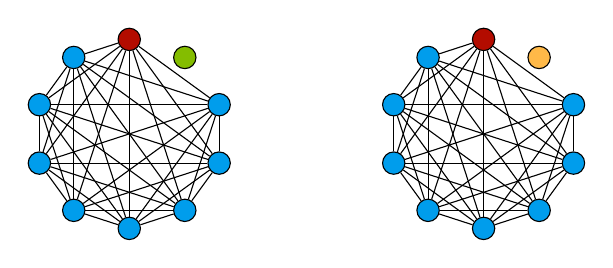
\begin{tikzpicture}[scale=0.5,every node/.style={font=\footnotesize}]
        \begin{scope}
            \newcount \myc
            \newcount \myd
            \newcount \mye
            \foreach \n in {1, ..., 8}{
                \myc=\n \advance\myc by -1 \multiply\myc by -360 \divide\myc by 10 \advance\myc by 18.0
                \node[draw, circle, fill=uofgcobalt, inner sep=0.5pt] (N\n) at (\the\myc:2.4) {\phantom{0}};
            }
            \node[draw, circle, fill=uofgpillarbox, inner sep=0.5pt] (N9) at (90.0:2.4) {\phantom{0}};
            \node[draw, circle, fill=uofglawn, inner sep=0.5pt] (N10) at (54.0:2.4) {\phantom{0}};

            \foreach \n in {1, ..., 8}{
                \myd=\n
                \myc=\n \advance\myc by 1
                \foreach \m in {\the\myc, ..., 9}{
                    \mye=\m
                    \draw (N\the\myd) -- (N\the\mye);
                }
            }
        \end{scope}
        \begin{scope}[xshift=9cm]
            \newcount \myc
            \newcount \myd
            \newcount \mye
            \foreach \n in {1, ..., 8}{
                \myc=\n \advance\myc by -1 \multiply\myc by -360 \divide\myc by 10 \advance\myc by 18.0
                \node[draw, circle, fill=uofgcobalt, inner sep=0.5pt] (N\n) at (\the\myc:2.4) {\phantom{0}};
            }
            \node[draw, circle, fill=uofgpillarbox, inner sep=0.5pt] (N9) at (90.0:2.4) {\phantom{0}};
            \node[draw, circle, fill=uofgpumpkin, inner sep=0.5pt] (N10) at (54.0:2.4) {\phantom{0}};

            \foreach \n in {1, ..., 8}{
                \myd=\n
                \myc=\n \advance\myc by 1
                \foreach \m in {\the\myc, ..., 9}{
                    \mye=\m
                    \draw (N\the\myd) -- (N\the\mye);
                }
            }
        \end{scope}
    \end{tikzpicture}}\only<1>{\begin{tikzpicture}[every node/.style={inner sep=0pt, outer sep=0pt, column sep=6pt}, ampersand replacement=\&]
        \matrix {
            \node [anchor=center] {}; \&
            \node [anchor=center] {\tiny $G(20, x, 1) \hookrightarrow G(150, y, 1)$}; \&
            \node [anchor=center] {\tiny $G(20, x, 2) \hookrightarrow G(150, y, 2)$}; \&
            \node [anchor=center] {\tiny $G(20, x, 5) \hookrightarrow G(150, y, 5)$}; \&
            \node [anchor=center] {\tiny $G(20, x, 20) \hookrightarrow G(150, y, 20)$}; \&
            \\[0.1cm]
                \node [anchor=center, inner sep=2pt] [rotate=90] {\tiny Glasgow}; \&
            \node [anchor=center] {\includegraphics{gen-graph-non-induced-nodes-20-150.pdf}}; \&
            \node [anchor=center] {\includegraphics{gen-graph-non-induced-nodes-20-l2-150.pdf}}; \&
            \node [anchor=center] {\includegraphics{gen-graph-non-induced-nodes-20-l5-150.pdf}}; \&
            \node [anchor=center] {\includegraphics{gen-graph-non-induced-nodes-20-l20-150.pdf}}; \&
            \\[0.1cm]
            \node [anchor=center, inner sep=2pt] [rotate=90] {\tiny VF2}; \&
            \node [anchor=center] {\includegraphics{gen-graph-vf2-non-induced-nodes-20-150.pdf}}; \&
            \node [anchor=center] {\includegraphics{gen-graph-vf2-non-induced-nodes-20-l2-150.pdf}}; \&
            \node [anchor=center] {\includegraphics{gen-graph-vf2-non-induced-nodes-20-l5-150.pdf}}; \&
            \node [anchor=center] {\includegraphics{gen-graph-vf2-non-induced-nodes-20-l20-150.pdf}}; \&
            \\
        };
\end{tikzpicture}}
\end{frame}

\begin{frame}{Constraint Programming versus Connectivity}
    \begin{center}\includegraphics{gen-graph-biiiig-data-pcms.pdf}\end{center}
\end{frame}

\begin{frame}{It's Not Just Graph Databases}
    \begin{displayquote}``There are (not so many) instances for which creation of a clear design is
        prohibitively slow in the current implementation that evaluates subgraph isomorphism with the
        VF2 algorithm \ldots Recent experiences with a few of these showed that the LAD algorithm was
    very fast in ruling out impossible matches, where VF2 took a long time.''\footnote{See McCreesh
    et al., JAIR 61(2018) for references}\end{displayquote}
\end{frame}

\begin{frame}{So What?}
    \begin{itemize}
        \item There's a lot more to hardness than worst-case complexity analysis.
        \item Understanding how algorithms behave is important.
        \item Maybe we should try doing some science?
    \end{itemize}
\end{frame}

{
    \usebackgroundtemplate{
        \tikz[overlay, remember picture]
        \node[at=(current page.south), anchor=south, inner
        sep=0pt]{\includegraphics[keepaspectratio=true, width=\paperwidth]{background2.jpg}};
    }

    \begin{frame}[plain,noframenumbering]
        \begin{tikzpicture}[remember picture, overlay]
            \node at (current page.north west) {
                \begin{tikzpicture}[remember picture, overlay]
                    \fill [fill=uofguniversityblue, anchor=north west] (0, 0) rectangle (\paperwidth, -2.6cm);
                \end{tikzpicture}
            };

            \node (logo) [anchor=north east, shift={(-0.6cm,-0.6cm)}] at (current page.north east) {
                
\includegraphics[keepaspectratio=true,scale=0.7]{UoG_keyline.pdf}
            };

            \node [anchor=north west, shift={(0.6cm,-0.8cm)}] at (current page.north west) {
                \textcolor{white}{\url{http://www.dcs.gla.ac.uk/~ciaran}}
            };

            \node [anchor=north west, shift={(0.6cm,-1.4cm)}] at (current page.north west) {
                    \textcolor{white}{\href{mailto:ciaran.mccreesh@glasgow.ac.uk}{\nolinkurl{ciaran.mccreesh@glasgow.ac.uk}}}
            };
        \end{tikzpicture}
    \end{frame}
}

\end{document}

